\documentclass[a4paper,11pt,oneside]{scrreprt}
\usepackage[latin1]{inputenc}
\usepackage[english]{babel}
\usepackage{graphicx}
\usepackage{float}
\usepackage{geometry}
\geometry{verbose,a4paper,tmargin=25mm,bmargin=25mm,lmargin=10mm,rmargin=10mm}
\usepackage{paralist}

\usepackage{paracol}

\usepackage{todonotes}

\usepackage{listings}
\lstset{language=Java,
	tabsize=2,
	showspaces=false,
	showtabs=false,
	breaklines=true,
	showstringspaces=false,
	breakatwhitespace=true,
	commentstyle=\color{pgreen},
	keywordstyle=\color{pblue},
	stringstyle=\color{pred},
	basicstyle=\footnotesize\ttfamily,
	moredelim=[il][\textcolor{pgrey}]{$$},
	moredelim=[is][\textcolor{pgrey}]{\%\%}{\%\%}
}

\usepackage{tikz}
\usetikzlibrary{calc,patterns,angles,quotes}

\usepackage{caption}
\usepackage{subcaption}
\usepackage{tabularx} % in the preamble

\usepackage{pdfpages}

\begin{document}


\begin{center}
	Submitted by Group 36
	
	\bigskip
	
	\begin{tabular}{c}
	Group Members: \\
	CETIN, Ulfet (391819); GRUCZKA, FILIP (413279);	LIPINSKI, Bartosz (413177) \\
	\end{tabular}

	\bigskip
	
	DIS1 WS 19/20 Assignment 6\\
	Visual Design
	
	%	(ordered on lastname basis)
\end{center}
\vspace{0cm}

\section*{Task 1}


\begin{figure}[H]
	\centering
	\begin{subfigure}{.5\textwidth}
		\centering
		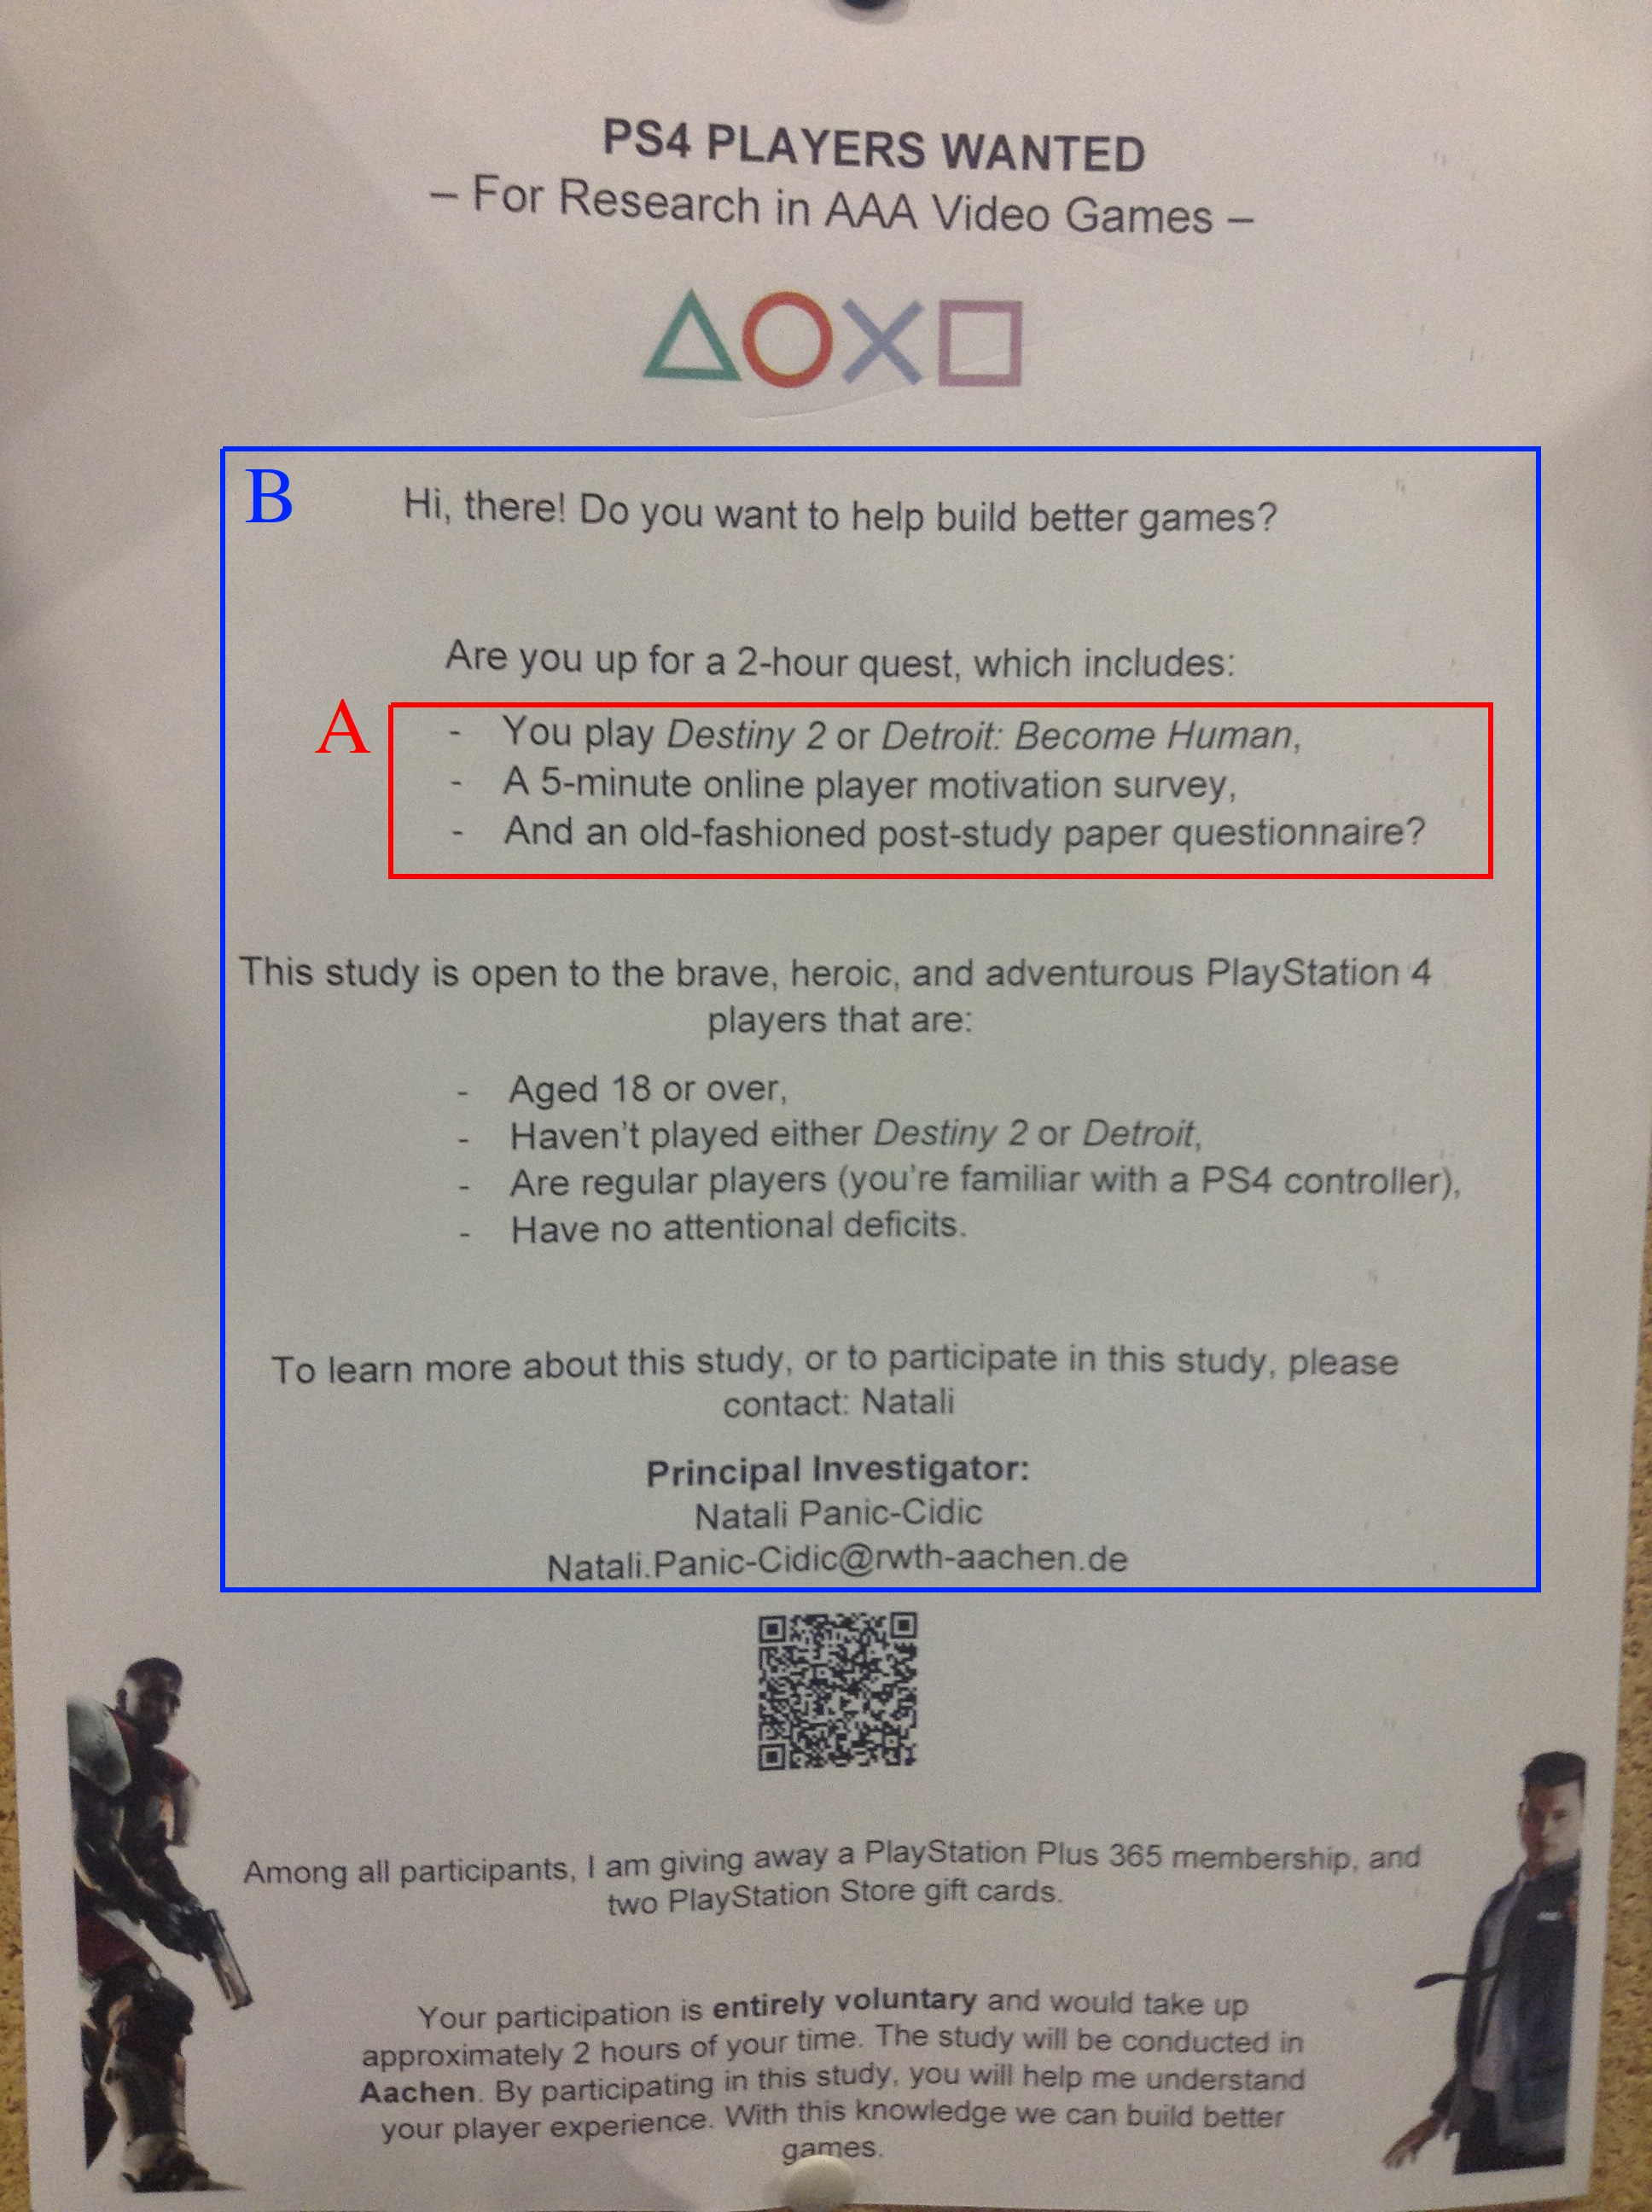
\includegraphics[clip, trim=0cm 0cm 0cm 0cm, scale=0.12]{./images/recruitment2.jpeg}
		\caption{PS4 Player Ad}
%		\label{fig:sub1}
	\end{subfigure}%
	\begin{subfigure}{.5\textwidth}
		\centering
		
\includegraphics[clip, trim=0cm 0cm 0cm 0cm, scale=0.53]{./images/proximity.jpg}
		\caption{Event Schedule}
%		\label{fig:sub2}
	\end{subfigure}
\end{figure}

\begin{figure}[H]
	

\begin{subfigure}{1\textwidth}
	\centering
	
\includegraphics[clip, trim=0cm 0cm 0cm 0cm, scale=0.4]{./images/kominiarze-ulotka.jpg}
	\caption{Chimney Sweep Leaflet}
	%		\label{fig:sub2}
\end{subfigure}
%	\caption{Video Lan Client (VLC) Right-Click Menu}
\label{fig:test}

\end{figure}

\begin{tabularx}{\textwidth}{|X|}
	\hline
		\textbf{Violations of Visual Design Principles}
		\\
	\hline
		\textbf{Violation \#1:} Contrast (PS4 Player Ad)\\
		Picture: \textbf{PS4 Player Ad:B}\\
		
		\\
		\textbf{Describe Violation:} Nearly no contrast, so many information with no distinction between nearly any text (titles have no contrast to the texts under them)
		
		
		\\
		\textbf{Why Bad?:} Makes it hard to distinguish between parts, and makes it hard to digest all the text. Assuming it has bold or larger subheaders (such as "Are you up for a 2-hour quest, which includes :" and "This study is open to brave, heroic, adventurous PS4 players that are:"), it would have been easier to understand the bill at the first glance. Although whitespace usage is not bad, he current form leads to more mental work distinguishing parts.
		
	\\
	\hline
	
		\textbf{Violation \#2:} Repetition (PS4 Player Ad)\\
		Picture: \textbf{PS4 Player Ad:B}
		
		\\
		\textbf{Describe Violation:} There is no consistent good repetition in the design. Aside from the same font size being used nearly everywhere, no part of the text and layout has been stepping forward to make a change in the view. This leads to dull-looking design. Note that there are tiny differences in the visual that steps forward like the main header "PS4 Players Wanted", and name of the investigator being bold, and two more; but those are few, thus, the style is repetitive in a negative sense, this repetitiveness does not help the user at all. 
		
		\\
		\textbf{Why Bad?:} User wants positive repetitiveness, and wants to know what to look at, how to continue reading text; in general, a good flow of style together with objects aligned well, like the CV example in the slides. In this, we have no such thing, the user is not 'guided' by the style that does not convey the idea of where to look. This is unstructured, or let's say repetitive in a bad manner that nothing gives out user any clue on what is important, where is the keypoints and so on.
		
	\\
	\hline	
	
		\textbf{Violation \#3:} Proximity (PS4 Player Ad)\\
		Picture: \textbf{PS4 Player Ad:A}
		
		\\
		\textbf{Describe Violation:} The list points(dashes) and the correspongding list items(texts) in the given bill have so much space in between them that them seem separate.
		
		\\
		\textbf{Why Bad?:} The list points and the list items observed as being separate does not help user digest them as coupled together, it is the other way, them seem separate. This leads to reading and observing difficulty, as they are not in their proximity, that is, not close enough.
		
		\\
		\hline	
	
	

	
\end{tabularx}\\

\begin{center}
	(continues from the next page)
	
\end{center}

\begin{tabularx}{\textwidth}{|X|}
	\hline	
	
	\textbf{Violation \#4:} Proximity (Event Schedule)
	Picture: \textbf{Event Schedule: C}
	\\
	\textbf{Describe Violation:} The middle (bold) part (C) is a schedule with 4 seperate meetings during an event and there is no space between them.
	
	\\
	\textbf{Why Bad?:} It is very hard to see that there are four seperate meetings there (C). That is because there are no gaps between lines so you have to read very carefully to distinguish one event from another. It is even more difficult, when in the last two meetings there are only informations about title and lecturer, which have bold font.
	
	\\
	\hline	
	
	\textbf{Violation \#5:} Allignment (Event Schedule)
	Picture: \textbf{Event Schedule: C}
	
	\\
	\textbf{Describe Violation:} The allignment in this schedule is centered that leads to difficulty with reading and makes schedule illogical. 
	
	\\
	\textbf{Why Bad?:} Not only the allignment on this leaflet makes reading difficult, it also has bad influance on aesthetic of it. It is especially bad in the middle part (C), where meeting schedule is included. Schedule should look like a list, which should be organized and logical, which is not a case with center allignment, that makes text messy and unpleasent for eye.
	
	\\
	\hline	
	
	\textbf{Violation \#6:} Allignment (Chimney Sweep Leaflet)
	Picture: \textbf{Chimney Sweep Leaflet: D}
	\\
	\textbf{Describe Violation:} Centered allignment makes the leaflet hard to read and would't encourage people to read it.
	
	\\
	\textbf{Why Bad?:} This leaflet is a very important message from chimney sweeps to people, that includes some information about necessary equipment, that everybody should have in order to not have a fire in their chimneys (D). However, the centered allignment and would make people unwilling to read it since it is very unpleasant for eye. Furthermore, it also causes that the most import message in this leaflet (the necessary equipment) is completely lost in a text in the middle part.
	
	\\
	\hline	
	
\end{tabularx}\\

\end{document}}
